Chapter \ref{chap:intro} introduced the unique characteristics of liquid-fuel
\glspl{MSR}
and highlighted the challenges of modeling liquid-fuel \glspl{MSR}, particularly
with legacy software designed for solid-fuel reactors. In addition, Chapter
\ref{chap:lit} summarized and discussed existing \gls{MSR} multiphysics simulation tools and
their capabilities. In this discussion, I noted the lack of capabilities for modeling control rod
movement in multiphysics tools for \glspl{MSR}. Chapter \ref{chap:moltres} illustrated general
features and physics models in Moltres and summarized previous work done with
Moltres for multiphysics modeling of \glspl{MSR}. The latter sections detailed
several limitations in \gls{MSR} multiphysics modeling with
Moltres, including the need for further verification of
Moltres' capabilities, a turbulence model for simulating turbulent flow, and a
control rod modeling capability for transient simulations. In turn,
Chapter \ref{chap:benchmark} detailed a verification study of Moltres for fast-spectrum
\gls{MSR} modeling capabilities by evaluating its performance
through the CNRS benchmark and comparing its results against other
\gls{MSR} simulation tools. Lastly, Chapter \ref{chap:hybrid} presented the theory and preliminary
1-D results of the novel hybrid $S_N$-diffusion method for improved control rod modeling over
standard neutron diffusion methods.

In this chapter, I will detail the proposed work to further verify and validate Moltres' \gls{MSR}
modeling capabilities, and I will describe the further enhancements to Moltres that I will
implement to address the
need for enhanced turbulence modeling and control rod modeling in Moltres. The
proposed work contributes towards improving on Moltres' capabilities for
multiphysics modeling of \glspl{MSR} and, by extension, of advanced reactors.
Section \ref{sec:vv-study} details the proposed \gls{VV} study of Moltres based on the \gls{MSRE}
pump start-up and coast-down experiments. Section \ref{sec:turb} describes the proposed
implementation of a \gls{RANS}-based turbulence model in Moltres. Section \ref{sec:devel-hybrid}
describes the proposed development and implementation of the hybrid $S_N$-diffusion in Moltres.
Lastly, Section \ref{sec:devel-conclusion} summarizes the chapter and describes the research impact
of my proposed work on \gls{MSR} modeling.

\section{Verification \& Validation Study Based on the MSRE Pump Start-up and Coast-Down
Experiments} \label{sec:vv-study}

In addition to the completed verification study described in Chapter \ref{chap:benchmark}, I will
perform a \gls{VV} study of Moltres based on the \gls{MSRE} transient flow-rate tests,
consisting of fuel pump start-up and coast-down experiments at zero power criticality. The changing
flow rates cause changes to the \gls{DNP} distribution and the \gls{DNF} in the core. During both
experiments, the reactivity effects of \gls{DNP} drift were measured by
allowing the flux servo controller to maintain criticality. The controller maintains core
criticality by adjusting the control rod position in response to the reactivity effects. The
reactivity effect over time can be calculated by comparing the various control rod positions
(Figure \ref{fig:msre-trans}) with the control rod worth curve (Figure \ref{fig:msre-rod})
obtained during earlier experiments. I aim to
reproduce the calculated reactivity curve with a Moltres model of the \gls{MSRE}.

\begin{figure}[htb!]
  \centering
  \begin{minipage}[t]{.49\textwidth}
    \centering
    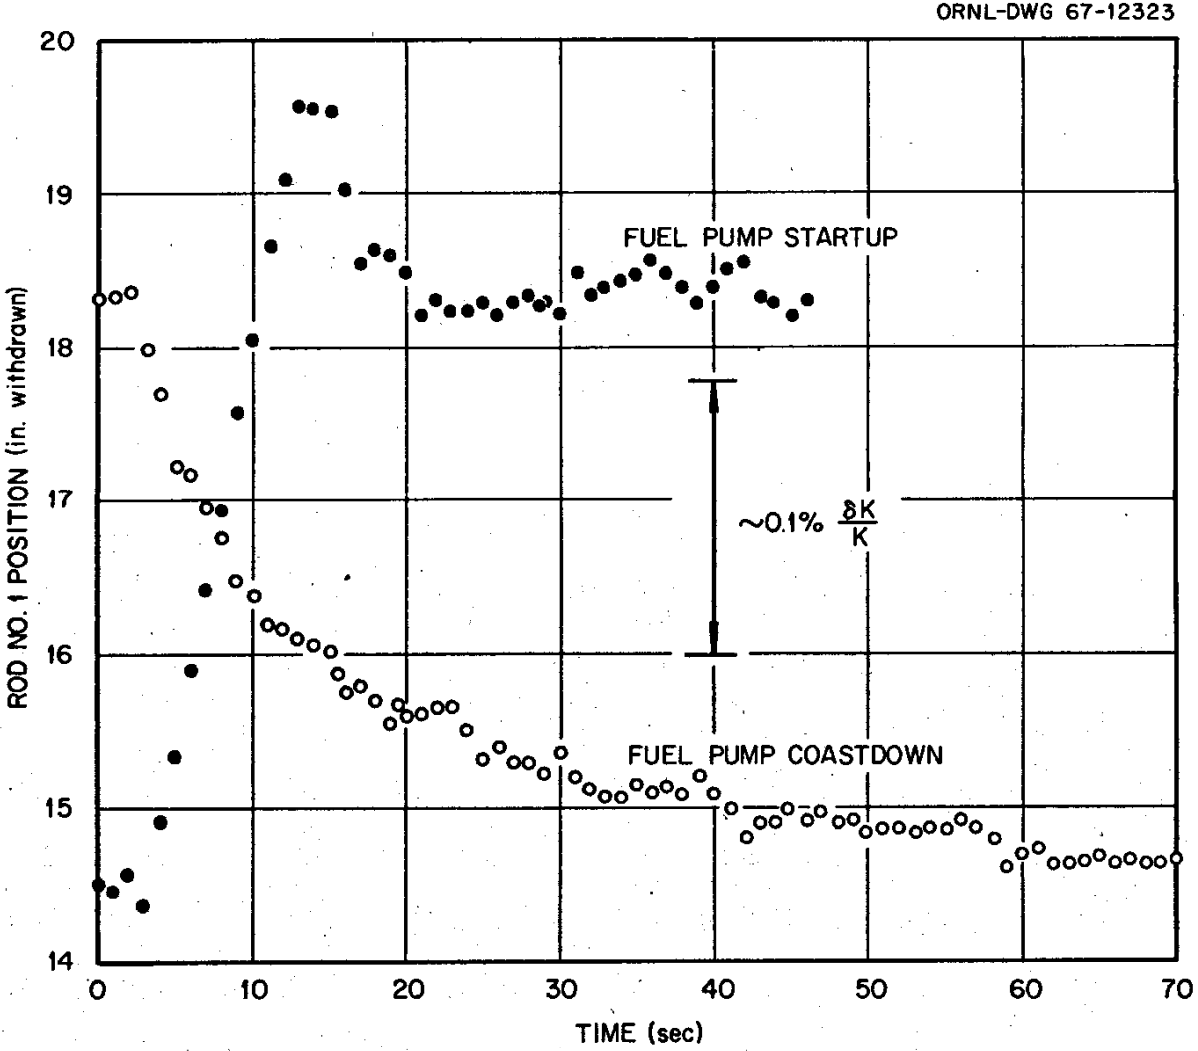
\includegraphics[width=\textwidth]{msre-transient}
    \caption{Control rod response to fuel pump start-up and coast-down
    \cite{prince_zero-power_1968}.}
    \label{fig:msre-trans}
  \end{minipage}
  \hfill
  \begin{minipage}[t]{.49\textwidth}
    \centering
    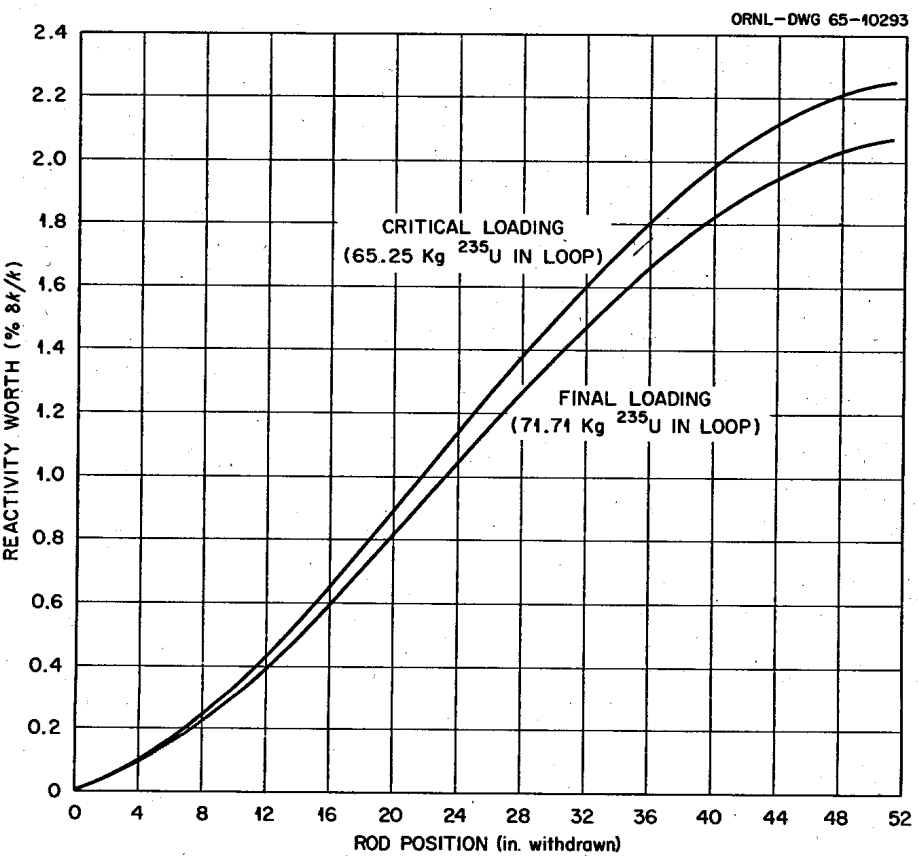
\includegraphics[width=\textwidth]{msre-rod-worth}
    \caption{Integral worth of control rod no. 1 \cite{prince_zero-power_1968}.}
    \label{fig:msre-rod}
  \end{minipage}
\end{figure}
%
\begin{figure}[htb!]
  \centering
  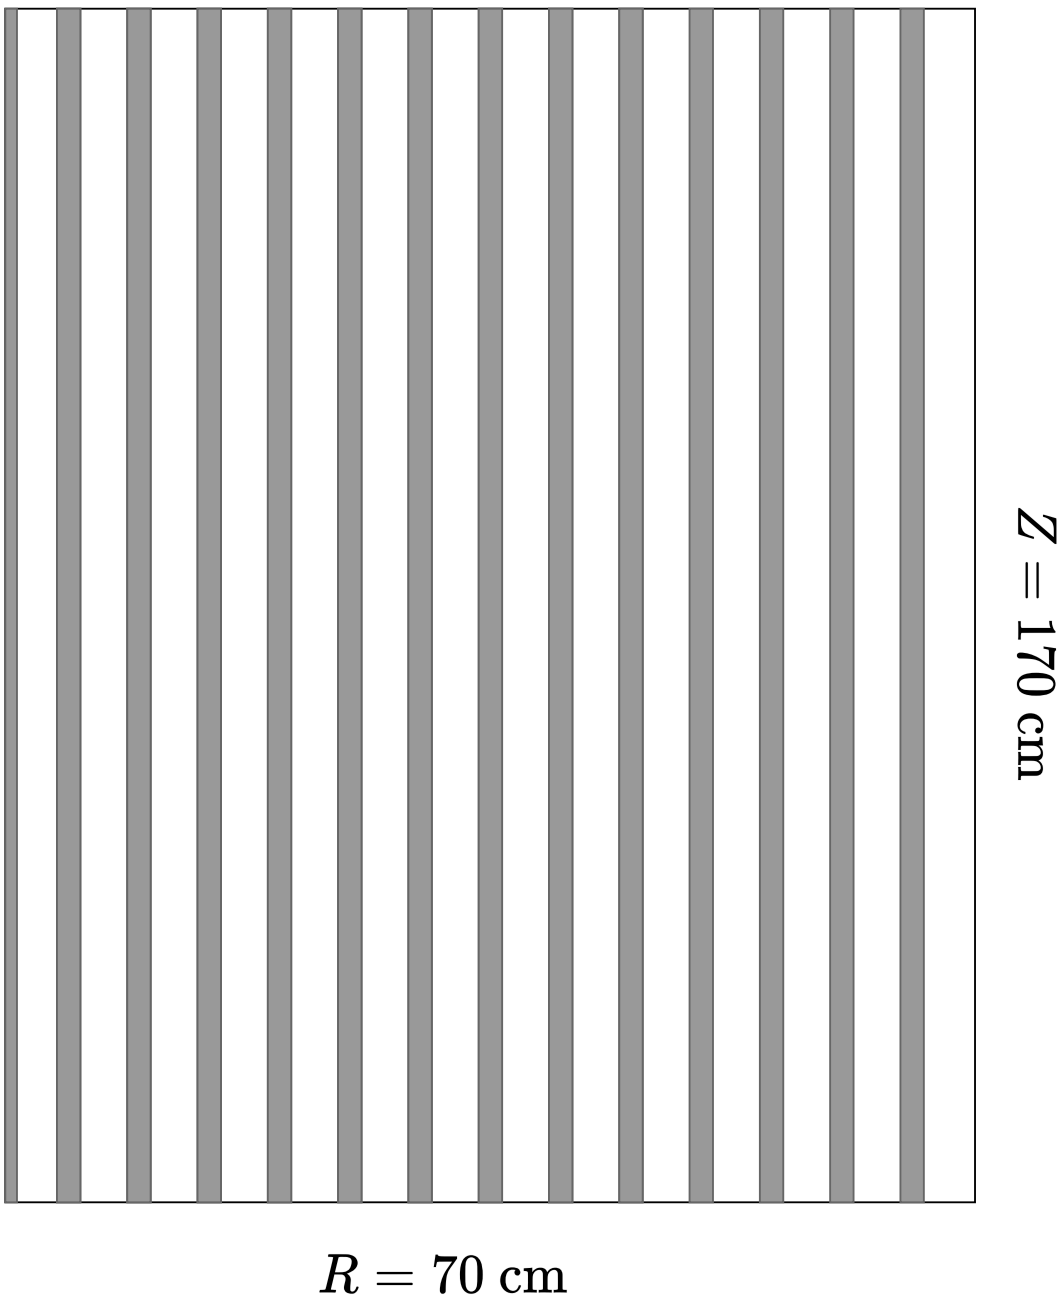
\includegraphics[width=.5\textwidth]{msre-2d}
  \caption{2-D axisymmetric model of the \gls{MSRE} to be used for the \gls{VV} study.}
  \label{fig:msre-2d}
\end{figure}

For this study, I will collaborate with Aaron Reynolds, the developer of QuasiMolto
\cite{reynolds_analysis_2023},
so that our software can be compared accurately. Therefore, Moltres
will be validated against \gls{MSRE} experimental data and verified against QuasiMolto simulation
results simultaneously. Both QuasiMolto and Moltres models of the \gls{MSRE} will be in R-Z
coordinates because QuasiMolto supports only 2-D R-Z \gls{MSR} modeling. Figure \ref{fig:msre-2d}
shows the 2-D axisymmetric model of the \gls{MSRE} that we intend to use
for this \gls{VV} study. The model omits the control rod in the \gls{MSRE}. Instead, we will
conduct $k$-eigenvalue calculations at every time-step to obtain the multiplication factor and
scale the \gls{DNP} source term. The salt flow speeds will be taken directly from available data in
the \gls{MSRE} report \cite{prince_zero-power_1968}. The datasets that we intend to compare between
QuasiMolto and Moltres for verification are:
%
\begin{itemize}
  \item Change in reactivity relative to the static (no flow) configuration over time during the
    pump start-up and coast-down transients
  \item Axial and radial neutron flux distributions of the static and steady-state (full flow)
    configurations
  \item Axial and radial \gls{DNP} distributions of the static and steady-state configurations
\end{itemize}

Since both QuasiMolto and Moltres will adopt the neutron diffusion method with the same flow
profile, we expect our results to be highly consistent with each other. We expect any discrepancies
between QuasiMolto and Moltres to be minor and due to differences in numerical discretization
schemes and routines. We will collaborate to eliminate errors arising from model misimplementation.

We also expect our reactivity data to be similar to the control rod response measured in Figure
\ref{fig:msre-trans}. However, our results are unlikely to match the experimental data exactly due
to known deficiencies in the physical \gls{MSRE} experimental setup and the simplifications we
adopted in our 2-D models. Among the model simplifications that we adopted, we expect the omission
of the upper and lower reactor plena to impact our results the most because the plena contain a
large volume of fuel salt above and below the fuel-graphite lattice. Therefore, as an extension, I
will consider exploring ways to include the plena in our models if our results deviate
significantly from the experimental data.

\section{Implementation of a RANS-Based Turbulence Model in Moltres} \label{sec:turb}

In Chapter \ref{chap:lit}, I presented requirements for \gls{MSR} modeling related to turbulence.
To address the current limitations, I will implement a Spalart-Allmaras turbulence model which
falls under the class of \gls{RANS}-based turbulence models. The
model will be implemented within the \gls{MOOSE} framework and
designed to be compatible with the fluid dynamics modeling infrastructure in
the existing \texttt{Navier-Stokes} module. This approach leverages the
advanced finite-element solver and multiphysics coupling capabilities in
\gls{MOOSE}.

I will
focus on verifying and validating its performance under specific flow conditions expected in
liquid-fuel \glspl{MSR}: wall-bounded turbulent flow with flow separation past
sharp changes in the flow channel geometry. The backward-facing step is a
widely known fluid dynamics problem commonly used to assess the accuracy of
turbulence model solvers \cite{lasher_computation_1992}.
The problem domain features a straight duct
on the left followed by a sudden back step in the lower wall which causes flow
separation. The flow eventually reattaches to the wall further downstream.
I will simulate and validate against experimental data from Driver \&
Seegmiller \cite{driver_features_1985}. The quantities of interest from their data that I plan to
use are the spatial distributions of the velocity components, turbulent
kinetic energy, and eddy viscosity, and the reattachment length of the
turbulent shear layer.

Potential issues that I may face include the lack of a crosswind diffusion stabilization scheme in
\gls{MOOSE} and the fact that local mass conservation is not guaranteed when modeling the
Navier-Stokes equations using the \gls{FEM} without special treatment. If these issues prove to be
insurmountable within a reasonable time frame, I will focus my efforts on adopting the mixing
length turbulence models currently available in \gls{MOOSE} or two-equation models which are in
active development with the recent \gls{FVM} implementation in \gls{MOOSE}. In this alternate
scenario, I will explore demonstrating coupled neutronics/thermal-hydraulics simulations with
turbulent flow modeling of the \gls{MSFR}.

\section{Development of a Novel Hybrid Method to Improve Control Rod Modeling in Moltres}
\label{sec:devel-hybrid}

In Chapter \ref{chap:hybrid}, I presented the theory and preliminary results of the hybrid
$S_N$-diffusion method for several 1-D \gls{MSRE}-inspired, graphite-moderated geometries. The
hybrid method generates \glspl{SVDC}, which provide pointwise corrections to the diffusion
sub-solver from
the $S_N$ sub-solver neutron current and flux gradient solutions. The hybrid method minimizes
computational costs by imposing the $S_N$ calculations on a small subdomain centered on the control
rod region and relaxing the $S_N$ sub-solver convergence tolerance since the neutron current and
flux gradient converges faster than the neutron flux. As intended,
the hybrid method provided better multiplication factor and neutron flux estimates over the
standard neutron diffusion method in systems containing strongly neutron-absorbing control rods.

In this section, I present a detailed description of the proposed work for the development and
implementation of the hybrid method in Moltres, the verification of the hybrid method against
reference OpenMC neutronics calculations, and the computational performance characterization of the
hybrid method.

\subsection{Development \& Implementation of the Hybrid Method}

The preliminary investigations in Chapter \ref{chap:hybrid} brought up three issues to be
addressed for the continued development of the hybrid $S_N$-diffusion method. The first issue
surrounds resolving \glspl{SVDC} near neutron flux peaks and troughs. The existing formulation
for \glspl{SVDC} in Eq. \ref{eq:svdc} are undefined at flux peaks and troughs due to division by
the flux gradient. I will explore alternative formulations to address this issue. For instance,
Tomatis \& Dall'Osso \cite{tomatis_application_2011} developed the formulation in Eq.
\ref{eq:tomatis} to address the same issue in their implementation of the Ronen method. Eq.
\ref{eq:tomatis} calculates corrections to the neutron streaming terms as additive
$\delta J$ terms. I will evaluate whether their formulation can be adapted to the hybrid
$S_N$-diffusion method. Otherwise, I plan to investigate similar additive correction formulations
for the hybrid $S_N$-diffusion method.

The second issue concerns the evaluation of appropriate correction regions and buffer zones for the
hybrid method. The correction region represents the problem domain of the $S_N$ sub-solver. It must
be large enough to provide sufficient transport correction in regions heavily influenced by the
control rod and to accommodate the discarding of inaccurate \glspl{SVDC} expected near the
boundary. I will investigate various test cases in 2-D and 3-D, similar to my preliminary work in
this report, to identify how various geometrical and material properties affect the minimum
required size of the correction region. For instance, my preliminary work showed that the
geometrical heterogeneity and optical thickness strongly affects the \gls{SVDC} distributions,
which are a measure of the amount of transport correction required. With my expected findings, I
will generate a set of criteria for determining the appropriate correction region size for a given
reactor geometry.

The last issue concerns the automatic evaluation of buffer zones which are regions near the
boundaries of the correction region where inaccurate \glspl{SVDC} are discarded. For the 1-D
problems, I set up an outward sweeping algorithm that compares the \glspl{SVDC} with the default
$P_1$-based diffusion coefficients. The implementation of this sweeping algorithm is less clear for
2-D and 3-D problems which feature more than two angular directions. I will tackle this issue
in conjunction with the second issue by analyzing the \gls{SVDC} distributions obtained from
2-D and 3-D test cases.

Naturally, the implementation and extension of the hybrid method in Moltres for 2-D and 3-D
modeling must precede my attempts at resolving the second and third issue. I will implement the
$S_N$ method with diffusion synthetic acceleration in Moltres or as a separate MOOSE-based
application. I will also implement supporting features for the coupling the $S_N$ solver with the
existing diffusion solver to run the hybrid method.

\subsection{Verification of the Hybrid Method}

I will verify the hybrid method against reference OpenMC calculations with several test cases
similar to the 1-D test cases in Chapter \ref{chap:hybrid}. The test cases will be various 2-D
and 3-D representations of \gls{MSRE}-inspired models with the fuel-graphite lattice, the control
rod, the air-filled rod guide tube, and reflectors. The verification study will include
permutations of the following factors:
%
\begin{itemize}
  \item Dimensionality (e.g, 2-D, 3-D)
  \item Geometrical symmetries and asymmetries related to the control rod position
  \item Static control rods at various levels of insertion
  \item Control rod material composition
\end{itemize}

\subsection{Computational Performance Characterization of the Hybrid Method}

I intend for the hybrid $S_N$-diffusion method to be tractable on small computing clusters for
time-dependent multiphysics simulations. Therefore, I will characterize the computational
performance of the hybrid method and compare it against the standard $S_N$ and neutron diffusion
methods. I expect the hybrid method to be faster than the standard $S_N$ method due to the small
correction region size relative to the full reactor geometry and the faster convergence of
\glspl{SVDC} relative to the neutron flux in the hybrid $S_N$ sub-solvers. I plan to perform the
characterization with some of the 2-D and 3-D verification study test cases.

In addition, I will evaluate the hybrid method's parallel scaling performance to identify potential
performance bottlenecks in the implementation. Good parallel scaling performance is essential for
leveraging on computational resources for large reactor simulations. I will run both weak and
strong scaling studies using some of the 2-D and 3-D test cases for this evaluation.

\section{Conclusion} \label{sec:devel-conclusion}

In this chapter, I detailed the proposed work to verify and validate Moltres' existing capabilities
for modeling \gls{DNP} drift and out-of-core decay in \glspl{MSR}, implement a \gls{RANS}-based
turbulence model in Moltres, and develop a hybrid $S_N$-diffusion method for improved control
rod modeling in Moltres. My work will extend the applicability of Moltres for a wider range of
MSR safety analyses involving turbulent flow and control rod effects. Most notably, the hybrid
method will enable Moltres users to run time-dependent multiphysics \gls{MSR} simulations with
control rod movement and address this technical gap in the existing literature. Through my work on
the hybrid method, I will also characterize and provide insights on neutron transport effects in
\gls{MSR} that are neglected by the neutron diffusion method.
